%%
%% Beginning of file 'sample.tex'
%%
%% Modified 2005 December 5
%%
%% This is a sample manuscript marked up using the
%% AASTeX v5.x LaTeX 2e macros.

%% The first piece of markup in an AASTeX v5.x document
%% is the \documentclass command. LaTeX will ignore
%% any data that comes before this command.

%% The command below calls the preprint style
%% which will produce a one-column, single-spaced document.
%% Examples of commands for other substyles follow. Use
%% whichever is most appropriate for your purposes.
%%
%%\documentclass[12pt,preprint]{aastex}

%% manuscript produces a one-column, double-spaced document:

\documentclass[manuscript]{../aastex52/aastex}

%% preprint2 produces a double-column, single-spaced document:

%% \documentclass[preprint2]{aastex}

%% Sometimes a paper's abstract is too long to fit on the
%% title page in preprint2 mode. When that is the case,
%% use the longabstract style option.

%% \documentclass[preprint2,longabstract]{aastex}

%% If you want to create your own macros, you can do so
%% using \newcommand. Your macros should appear before
%% the \begin{document} command.
%%
%% If you are submitting to a journal that translates manuscripts
%% into SGML, you need to follow certain guidelines when preparing
%% your macros. See the AASTeX v5.x Author Guide
%% for information.

\newcommand{\vdag}{(v)^\dagger}
\newcommand{\myemail}{skywalker@galaxy.far.far.away}

%% You can insert a short comment on the title page using the command below.

\slugcomment{Not to appear in Nonlearned J., 45.}

%% If you wish, you may supply running head information, although
%% this information may be modified by the editorial offices.
%% The left head contains a list of authors,
%% usually a maximum of three (otherwise use et al.).  The right
%% head is a modified title of up to roughly 44 characters.
%% Running heads will not print in the manuscript style.

\shorttitle{Collapsed Cores in Globular Clusters}
\shortauthors{Djorgovski et al.}

%% This is the end of the preamble.  Indicate the beginning of the
%% paper itself with \begin{document}.

\begin{document}

%% LaTeX will automatically break titles if they run longer than
%% one line. However, you may use \\ to force a line break if
%% you desire.

\title{Power law properties of Fourier power spectra and their
  implications for coronal seismology and coronal heating.}

%% Use \author, \affil, and the \and command to format
%% author and affiliation information.
%% Note that \email has replaced the old \authoremail command
%% from AASTeX v4.0. You can use \email to mark an email address
%% anywhere in the paper, not just in the front matter.
%% As in the title, use \\ to force line breaks.

\author{J. Ireland}
\affil{ADNET Systems, Inc.,NASA Goddard Space Flight Center, MC. 671.1 Greenbelt, MD
  20771, USA. }
\email{jack.ireland@nasa.gov}

\author{R. T. J. McAteer}
\affil{Department of Astronomy, New Mexico State University, Las
  Cruces, NM}

\and

\author{A. R. Inglis}
\affil{Catholic University of America / NASA Goddard Space Flight Center, MC. 671.1 Greenbelt, MD
  20771, USA.}

%% Mark off your abstract in the ``abstract'' environment. In the manuscript
%% style, abstract will output a Received/Accepted line after the
%% title and affiliation information. No date will appear since the author
%% does not have this information. The dates will be filled in by the
%% editorial office after submission.

\begin{abstract}
The Fourier power spectra of regions of the solar corona are
investigated using AIA 171\AA\ and 193\AA\ data.  It is shown that the
Fourier power spectra in all the regions show a power law behaviour
approximately.  This suggests that in many parts of the corona a
background model consisting of white noise and a trend cannot be
assumed when analyzing for the presence of oscillations in the corona.
Further, it is shown that the observed power law power spectrum is
consistent with that expected from summing a distribution of
exponentially decaying emission events along the line of sight.  This
is consistent with the notion that the corona is heated everywhere by
small energy deposition events, such as nanoflares.
\end{abstract}

%% Keywords should appear after the \end{abstract} command. The uncommented
%% example has been keyed in ApJ style. See the instructions to authors
%% for the journal to which you are submitting your paper to determine
%% what keyword punctuation is appropriate.

\keywords{???}

%% From the front matter, we move on to the body of the paper.
%% In the first two sections, notice the use of the natbib \citep
%% and \citet commands to identify citations.  The citations are
%% tied to the reference list via symbolic KEYs. The KEY corresponds
%% to the KEY in the \bibitem in the reference list below. We have
%% chosen the first three characters of the first author's name plus
%% the last two numeral of the year of publication as our KEY for
%% each reference.


%% Authors who wish to have the most important objects in their paper
%% linked in the electronic edition to a data center may do so by tagging
%% their objects with \objectname{} or \object{}.  Each macro takes the
%% object name as its required argument. The optional, square-bracket 
%% argument should be used in cases where the data center identification
%% differs from what is to be printed in the paper.  The text appearing 
%% in curly braces is what will appear in print in the published paper. 
%% If the object name is recognized by the data centers, it will be linked
%% in the electronic edition to the object data available at the data centers  
%%
%% Note that for sources with brackets in their names, e.g. [WEG2004] 14h-090,
%% the brackets must be escaped with backslashes when used in the first
%% square-bracket argument, for instance, \object[\[WEG2004\] 14h-090]{90}).
%%  Otherwise, LaTeX will issue an error. 

\section{Introduction}

The solar corona is observed to support many different oscillatory
phenomena.



\section{Observations}\label{sec:obs}

Data was obtained from SDO-AIA using the Lockheed Martin Solar
Astrophysics cutout service (http://lmsal.com/get\_aia\_data/).  Six
hours of image data at 12 second cadence was selected in the 171\AA
and 193\AA\ wavebands (2012-09-23 00:00 - 06:00 UT, 1800 images per
waveband).  These wavebands were selected in order to obtain a wide
range of approximate temperatures in the solar corona.

The downloaded cutout data was prepared for analysis using the
SolarSoft / IDL routines READ\_SDO and AIA\_PREP.  These procedures
move the downloaded level 1.0 FITS files to level 1.5 FITS files.  All
further processing from this point was performed in the SunPy 0.4
(http://www.sunpy.org) data analysis environment.  Images were
de-rotated to compensate for solar rotation, based on the center of
the field of view of each image.  After de-rotation, each image layer
was co-registered with the image half way through the dataset, at
approximately 03:00 UT.

\section{Analysis}\label{sec:anal}

We wish to analyze the frequency content of these resulting datacubes
as a function of spatial location.  Four locations were chosen in the
data representing four different types of physical locations in the
solar atmosphere.  These were a quiet Sun region, a region that lies
on top of a sunspot, a footpoint region, and a coronal moss region.
Figures \ref{fig:loc171193} show the location of the regions on sample
images from the time range considered.

\begin{figure}
\label{fig:loc171}
\plottwo{shutdownfun3_6hr_disk_1.5_171.eps}{shutdownfun3_6hr_disk_1.5_171.eps}
\caption{171 and 193}
\end{figure}

Consider the emission from a single pixel, $I(t)$.  The Fourier power
spectrum for this emission was calculated as follows.  First, the
time-series was normalized by calculating $(I(t) - <I(t)>)/<I(t)>$.
This normalizes the emission.  Secondly, the normalized time-series
was apodized using the Hanning window, reducing ringing effects.  This
results in a time-series from which its Fourier power spectrum was
analyzed. 

Figures \ref{fig:compare171193} show example power spectra, plotted using
a log-log scale, from a single location inside each of the regions
shown in Figures \ref{fig:loc171} and \ref{fig:loc193}.  The shape of
the power spectra indicate that the Fourier power approximately
follows a power law at lower frequencies and flattens out at higher
frequencies.

\begin{figure}
\label{fig:compare171193}
\plottwo{loopfootpoints.centralpower.eps}{qs.centralpower.eps}
\plottwo{sunspot.centralpower.eps}{moss.centralpower.eps}
\caption{Log-log plot of the Fourier power of a time-series at the AIA
  pixel overlying a randomly chosen pixel in each of the regions
  considered (see Figures \protect\ref{fig:loc171} and
  \protect\ref{fig:loc193}).  The vertical black lines indicate the 3
  and 5 minute frequencies.}
\end{figure}


Figures \ref{fig:dist171} and \ref{fig:dist193} show the distributions
of the logarithm of the Fourier power for certain frequencies in the
spectrum.  The distributions all approximately follow a normal
distribution.  This indicates that the power in each each at each
frequency is approximately log-normally distributed.  This observation
guides the choice of how to average the power spectrum over each of
the selected physical regions.  Since the Fourier power is
log-normally distributed, the arithmetic mean of the Fourier power is
biased by the very largest powers.  Hence the mean of the logarithm of
the Fourier power is considered, which is equivalent to the geometric
mean of the Fourier power.

\begin{figure}
\label{fig:dist171}

\caption{}
\end{figure}

\begin{figure}
\label{fig:dist193}

\caption{}
\end{figure}

These geometric mean Fourier power spectra are shown in Figures
\ref{fig:geom171} and \ref{fig:geom193}, for each of the physical
regions considered.  It is clear that the Fourier power spectra
exhibit power-law like characteristics.  

\begin{figure}
\label{fig:geom171}

\caption{}
\end{figure}

\begin{figure}
\label{fig:geom193}

\caption{}
\end{figure}

The results for the quiet Sun, loop footpoints and sunspot regions
suggest a power-law power spectrum.  This can be modeled as
\begin{equation}
\label{eq:pwrlaw}
P_{0}(f) = Af^{-n} + C,
\end{equation}
where $A>0$ is a proportionality constant, $n>0$ is the power law
index, and $C>0$ describes the high-frequency Fourier power.

The moss results for 171\AA\ and 193\AA\ are notably different from
the other results.  In comparison to the general trend observed in
other regions, there appears to be excess Fourier power in the range
1-10 mHz.  Previous studies (???) have shown that the moss is a source
of uncorrelated and incoherent Fourier power.  This suggests that a
second model for these regions should be considered.  The spectrum
$P_{1}$ where
\begin{equation}
\label{eq:pwrlawbunp}
\ln P_{1}(f) = P_{0} + \alpha\exp\left[-\frac{(\ln(f)-\beta)^{2}}{2\sigma^{2}}\right]
\end{equation}
contains the previous power law dependence, plus the second term,
modelling the excess power.  

\subsection{Comparing power spectra models}\label{ssec:twomodels}




\section{Discussion}
The presence of a power law Fourier spectrum in coronal emission poses
questions about how that emission is formed.  The power law power
spectrum also has implications for the detection of narrow frequency
band oscillations against such a background emission, which is the
purview of coronal seismology.  We discuss these two topics in the
sections below.


\subsection{Coronal seismology and the effect of background assumptions}
\label{ssec:corseis}

Section \ref{sec:results} demonstrates the presence of a red
noise-like signal in two of the most commonly used wavebands for
coronal seismology, SDO-AIA 171\AA\ and 193\AA.  The observed spectra
generally show a power law-like behavior at time-scales of interest in
coronal seismology, and longer.  Coronal moss regions seem to show
slightly higher emission than a background power-law at a limited
range of frequencies.  However, this does not change the power-law
like nature of the emission - the power spectrum is essentially scale
free on average.  Therefore, on average, there is little guidance to
be had from coronal Fourier power spectra that can be used to pick a
time-scale that can be used to remove a background trend.

If there is no time-scale that can be used to remove a background
trend, then the time-series has to be analyzed without this processing
step.  Here too, the red-noise nature of the emission can cause
problems in attempting to analyze for the presence of narrow frequency
band oscillations.  Such oscillations are thought to be indicative of
waves in the solar atmosphere.

\begin{figure}
\epsscale{.80}
\plotone{white_red_compare.eps}
\caption{Comparison of the effect of assuming a white or red noise
  background on the detection of an oscillatory signal for simulated
  time-series.  Plot (a) shows the simulated time-series, generated
  from a power spectrum \protect$P(f)\approx f^{-1.77}$ and no
  explicit oscillation included.  Plot (b) shows the wavelet power
  spectrum with the cone-of-influence (shaded area) and regions above
  the 95\% confidence level, assuming a white-noise (Gaussian)
 background .  Plot (c) shows the global wavelet power spectrum for
  this wavelet transform.  Plots (d) and (e) are the same as plots (b)
  and (c) under the assumption of a red-noise background.\label{fig:comparison}}
\end{figure}

Figure \ref{fig:comparison} shows how a red-noise power spectrum can
be mistakenly thought to contain an oscillatory signal.  The time
series (Figure \ref{fig:comparison}(a)) is constructed from a power
spectrum $P(f)\approx f^{-1.77}$ with no explicit oscillatory content,
following the construction procedure of \cite{vaughan2010}.  Figure
\ref{fig:comparison}(b) shows that the assumption of a white-noise
background and a 95\% confidence level leads to the positive detection
of significant oscillatory power in this time series. Figure
\ref{fig:comparison}(c) shows that the assumption of a red-noise
background with the same confidence level significantly reduces the
area for which a detection may be claimed.  This simulated data, along
with the results of Section \ref{sec:results}, suggest that when
examining the wavelet transforms of time-series for wave packets, a
background red-noise power spectrum should be assumed, along with
higher confidence levels, in order to minimize the effects of
mistakenly identifying red-noise as evidence for an oscillatory
signal.

The foregoing discusses the implications of red-noise power spectra
for the detection of narrow-frequency band oscillations when looking
at single time-series.  The advantage of AIA is that there is more
than one time-series to consider.  Evidence for the presence of a wave
in the corona is much stronger if it can be shown that narrow
frequency-band oscillations occur significantly above a red-noise
background signal in several neighboring pixels.


\subsection{Nature of the power law power spectrum}\label{ssec:nplps}


\section{Conclusions}\label{sec:conc}


%% If you wish to include an acknowledgments section in your paper,
%% separate it off from the body of the text using the \acknowledgments
%% command.

%% Included in this acknowledgments section are examples of the
%% AASTeX hypertext markup commands. Use \url without the optional [HREF]
%% argument when you want to print the url directly in the text. Otherwise,
%% use either \url or \anchor, with the HREF as the first argument and the
%% text to be printed in the second.

\acknowledgments

We are grateful to the developers of SSWIDL \cite{}, SunPy \cite{},
PyMC \cite{} and matplotlib \cite{} for providing data preparation,
manipulation, analysis and display packages.  This work was supported
by the NASA....

%% To help institutions obtain information on the effectiveness of their
%% telescopes, the AAS Journals has created a group of keywords for telescope
%% facilities. A common set of keywords will make these types of searches
%% significantly easier and more accurate. In addition, they will also be
%% useful in linking papers together which utilize the same telescopes
%% within the framework of the National Virtual Observatory.
%% See the AASTeX Web site at http://aastex.aas.org/
%% for information on obtaining the facility keywords.

%% After the acknowledgments section, use the following syntax and the
%% \facility{} macro to list the keywords of facilities used in the research
%% for the paper.  Each keyword will be checked against the master list during
%% copy editing.  Individual instruments or configurations can be provided 
%% in parentheses, after the keyword, but they will not be verified.

{\it Facilities:} \facility{Nickel}, \facility{HST (STIS)}, \facility{CXO (ASIS)}.

%% Appendix material should be preceded with a single \appendix command.
%% There should be a \section command for each appendix. Mark appendix
%% subsections with the same markup you use in the main body of the paper.

%% Each Appendix (indicated with \section) will be lettered A, B, C, etc.
%% The equation counter will reset when it encounters the \appendix
%% command and will number appendix equations (A1), (A2), etc.

\appendix

\section{Appendix material}

Consider once again a task that computes profile parameters for a modified
Lorentzian of the form
\begin{equation}
I = \frac{1}{1 + d_{1}^{P (1 + d_{2} )}}
\end{equation}
where
\begin{mathletters}
\begin{displaymath}
d_{1} = \frac{3}{4} \sqrt{ \left( \begin{array}{c} \frac{x_{1}}{R_{maj}}
\end{array} \right) ^{2} +
\left( \begin{array}{c} \frac{y_{1}}{R_{min}} \end{array} \right) ^{2} }
\end{displaymath}
\begin{equation}
d_{2} = \case{3}{4} \sqrt{ \left( \begin{array}{c} \frac{x_{1}}{P R_{maj}}
\end{array} \right) ^{2} +
\left( \begin{array}{c} \case{y_{1}}{P R_{min}} \end{array} \right) ^{2} }
\end{equation}
\begin{eqnarray}
x_{1} & = & (x - x_{0}) \cos \Theta + (y - y_{0}) \sin \Theta \\
y_{1} & = & -(x - x_{0}) \sin \Theta + (y - y_{0}) \cos \Theta
\end{eqnarray}
\end{mathletters}

For completeness, here is one last equation.
\begin{equation}
e = mc^2
\end{equation}

%% The reference list follows the main body and any appendices.
%% Use LaTeX's thebibliography environment to mark up your reference list.
%% Note \begin{thebibliography} is followed by an empty set of
%% curly braces.  If you forget this, LaTeX will generate the error
%% "Perhaps a missing \item?".
%%
%% thebibliography produces citations in the text using \bibitem-\cite
%% cross-referencing. Each reference is preceded by a
%% \bibitem command that defines in curly braces the KEY that corresponds
%% to the KEY in the \cite commands (see the first section above).
%% Make sure that you provide a unique KEY for every \bibitem or else the
%% paper will not LaTeX. The square brackets should contain
%% the citation text that LaTeX will insert in
%% place of the \cite commands.

%% We have used macros to produce journal name abbreviations.
%% AASTeX provides a number of these for the more frequently-cited journals.
%% See the Author Guide for a list of them.

%% Note that the style of the \bibitem labels (in []) is slightly
%% different from previous examples.  The natbib system solves a host
%% of citation expression problems, but it is necessary to clearly
%% delimit the year from the author name used in the citation.
%% See the natbib documentation for more details and options.

\begin{thebibliography}{}
\bibitem[Auri\`ere(1982)]{aur82} Auri\`ere, M.  1982, \aap,
    109, 301
\bibitem[Canizares et al.(1978)]{can78} Canizares, C. R.,
    Grindlay, J. E., Hiltner, W. A., Liller, W., \&
    McClintock, J. E.  1978, \apj, 224, 39
\bibitem[Djorgovski \& King(1984)]{djo84} Djorgovski, S.,
    \& King, I. R.  1984, \apjl, 277, L49
\bibitem[Hagiwara \& Zeppenfeld(1986)]{hag86} Hagiwara, K., \&
    Zeppenfeld, D.  1986, Nucl.Phys., 274, 1
\bibitem[Harris \& van den Bergh(1984)]{har84} Harris, W. E.,
    \& van den Bergh, S.  1984, \aj, 89, 1816
\bibitem[H\`enon(1961)]{hen61} H\'enon, M.  1961, Ann.d'Ap., 24, 369
\bibitem[Heiles \& Troland(2003)]{heiles03} Heiles, C. \& Troland, T. H., 2003, \apjs, preprint doi:10.1086/381753
\bibitem[Kim, Ostricker, \& Stone(2003)]{kim03} Kim, W.-T.,  Ostriker, E., \& Stone, J. M., 2003, \apj, 599, 1157
\bibitem[King(1966)]{kin66}  King, I. R.  1966, \aj, 71, 276
\bibitem[King(1975)]{kin75}  King, I. R.  1975, Dynamics of
    Stellar Systems, A. Hayli, Dordrecht: Reidel, 1975, 99
\bibitem[King et al.(1968)]{kin68}  King, I. R., Hedemann, E.,
    Hodge, S. M., \& White, R. E.  1968, \aj, 73, 456
\bibitem[Kron et al.(1984)]{kro84} Kron, G. E., Hewitt, A. V.,
    \& Wasserman, L. H.  1984, \pasp, 96, 198
\bibitem[Lynden-Bell \& Wood(1968)]{lyn68} Lynden-Bell, D.,
    \& Wood, R.  1968, \mnras, 138, 495
\bibitem[Newell \& O'Neil(1978)]{new78} Newell, E. B.,
    \& O'Neil, E. J.  1978, \apjs, 37, 27
\bibitem[Ortolani et al.(1985)]{ort85} Ortolani, S., Rosino, L.,
    \& Sandage, A.  1985, \aj, 90, 473
\bibitem[Peterson(1976)]{pet76} Peterson, C. J.  1976, \aj, 81, 617
\bibitem[Rudnick et al.(2003)]{rudnick03} Rudnick, G. et al., 2003, \apj, 599, 847
\bibitem[Spitzer(1985)]{spi85} Spitzer, L.  1985, Dynamics of
    Star Clusters, J. Goodman \& P. Hut, Dordrecht: Reidel, 109
\bibitem[Treu et al.(2003)]{treu03} Treu, T. et al., 2003, \apj, 591, 53
\end{thebibliography}

\clearpage

%% Use the figure environment and \plotone or \plottwo to include
%% figures and captions in your electronic submission.
%% To embed the sample graphics in
%% the file, uncomment the \plotone, \plottwo, and
%% \includegraphics commands
%%
%% If you need a layout that cannot be achieved with \plotone or
%% \plottwo, you can invoke the graphicx package directly with the
%% \includegraphics command or use \plotfiddle. For more information,
%% please see the tutorial on "Using Electronic Art with AASTeX" in the
%% documentation section at the AASTeX Web site, http://aastex.aas.org/
%%
%% The examples below also include sample markup for submission of
%% supplemental electronic materials. As always, be sure to check
%% the instructions to authors for the journal you are submitting to
%% for specific submissions guidelines as they vary from
%% journal to journal.

%% This example uses \plotone to include an EPS file scaled to
%% 80% of its natural size with \epsscale. Its caption
%% has been written to indicate that additional figure parts will be
%% available in the electronic journal.

\clearpage

%% Here we use \plottwo to present two versions of the same figure,
%% one in black and white for print the other in RGB color
%% for online presentation. Note that the caption indicates
%% that a color version of the figure will be available online.
%%

\begin{figure}
\plottwo{f2.eps}{f2_color.eps}
\caption{A panel taken from Figure 2 of \citet{rudnick03}. 
See the electronic edition of the Journal for a color version 
of this figure.\label{fig2}}
\end{figure}

%% This figure uses \includegraphics to scale and rotate the still frame
%% for an mpeg animation.

\begin{figure}
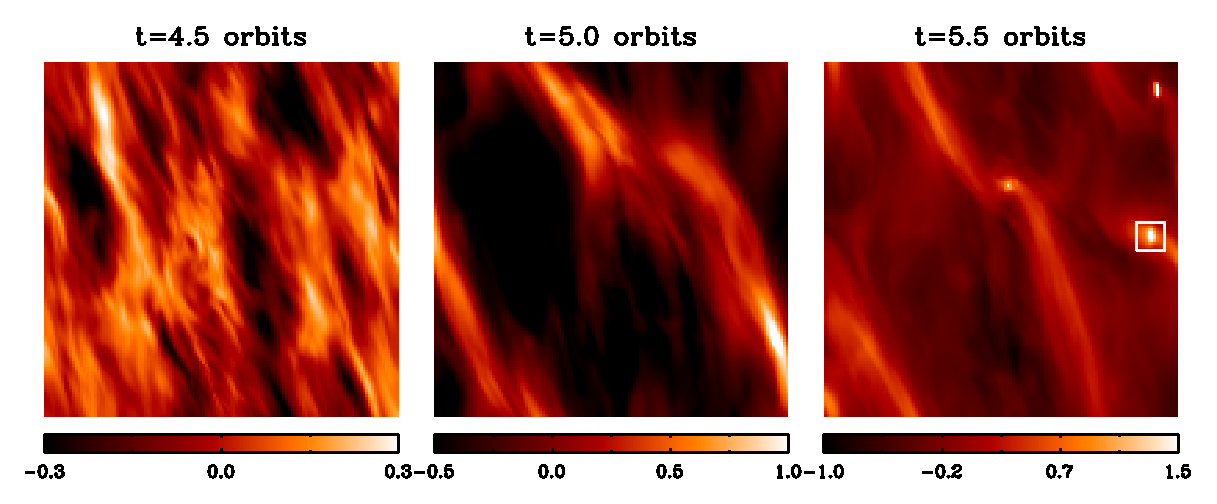
\includegraphics[angle=90,scale=.50]{f3.eps}
\caption{Animation still frame taken from \citet{kim03}.
This figure is also available as an mpeg
animation in the electronic edition of the
{\it Astrophysical Journal}.}
\end{figure}

%% If you are not including electonic art with your submission, you may
%% mark up your captions using the \figcaption command. See the
%% User Guide for details.
%%
%% No more than seven \figcaption commands are allowed per page,
%% so if you have more than seven captions, insert a \clearpage
%% after every seventh one.

%% Tables should be submitted one per page, so put a \clearpage before
%% each one.

%% Two options are available to the author for producing tables:  the
%% deluxetable environment provided by the AASTeX package or the LaTeX
%% table environment.  Use of deluxetable is preferred.
%%

%% Three table samples follow, two marked up in the deluxetable environment,
%% one marked up as a LaTeX table.

%% In this first example, note that the \tabletypesize{}
%% command has been used to reduce the font size of the table.
%% We also use the \rotate command to rotate the table to
%% landscape orientation since it is very wide even at the
%% reduced font size.
%%
%% Note also that the \label command needs to be placed
%% inside the \tablecaption.

%% This table also includes a table comment indicating that the full
%% version will be available in machine-readable format in the electronic
%% edition.

\clearpage

\begin{deluxetable}{ccrrrrrrrrcrl}
\tabletypesize{\scriptsize}
\rotate
\tablecaption{Sample table taken from \citet{treu03}\label{tbl-1}}
\tablewidth{0pt}
\tablehead{
\colhead{POS} & \colhead{chip} & \colhead{ID} & \colhead{X} & \colhead{Y} &
\colhead{RA} & \colhead{DEC} & \colhead{IAU$\pm$ $\delta$ IAU} &
\colhead{IAP1$\pm$ $\delta$ IAP1} & \colhead{IAP2 $\pm$ $\delta$ IAP2} &
\colhead{star} & \colhead{E} & \colhead{Comment}
}
\startdata
0 & 2 & 1 & 1370.99 & 57.35    &   6.651120 &  17.131149 & 21.344$\pm$0.006  & 2
4.385$\pm$0.016 & 23.528$\pm$0.013 & 0.0 & 9 & -    \\
0 & 2 & 2 & 1476.62 & 8.03     &   6.651480 &  17.129572 & 21.641$\pm$0.005  & 2
3.141$\pm$0.007 & 22.007$\pm$0.004 & 0.0 & 9 & -    \\
0 & 2 & 3 & 1079.62 & 28.92    &   6.652430 &  17.135000 & 23.953$\pm$0.030  & 2
4.890$\pm$0.023 & 24.240$\pm$0.023 & 0.0 & - & -    \\
0 & 2 & 4 & 114.58  & 21.22    &   6.655560 &  17.148020 & 23.801$\pm$0.025  & 2
5.039$\pm$0.026 & 24.112$\pm$0.021 & 0.0 & - & -    \\
0 & 2 & 5 & 46.78   & 19.46    &   6.655800 &  17.148932 & 23.012$\pm$0.012  & 2
3.924$\pm$0.012 & 23.282$\pm$0.011 & 0.0 & - & -    \\
0 & 2 & 6 & 1441.84 & 16.16    &   6.651480 &  17.130072 & 24.393$\pm$0.045  & 2
6.099$\pm$0.062 & 25.119$\pm$0.049 & 0.0 & - & -    \\
0 & 2 & 7 & 205.43  & 3.96     &   6.655520 &  17.146742 & 24.424$\pm$0.032  & 2
5.028$\pm$0.025 & 24.597$\pm$0.027 & 0.0 & - & -    \\
0 & 2 & 8 & 1321.63 & 9.76     &   6.651950 &  17.131672 & 22.189$\pm$0.011  & 2
4.743$\pm$0.021 & 23.298$\pm$0.011 & 0.0 & 4 & edge \\
\enddata
%% Text for table notes should follow after the \enddata but before
%% the \end{deluxetable}. Make sure there is at least one \tablenotemark
%% in the table for each \tablenotetext.
\tablecomments{Table \ref{tbl-1} is published in its entirety in the 
electronic edition of the {\it Astrophysical Journal}.  A portion is 
shown here for guidance regarding its form and content.}
\tablenotetext{a}{Sample footnote for table~\ref{tbl-1} that was generated
with the deluxetable environment}
\tablenotetext{b}{Another sample footnote for table~\ref{tbl-1}}
\end{deluxetable}

%% If you use the table environment, please indicate horizontal rules using
%% \tableline, not \hline.
%% Do not put multiple tabular environments within a single table.
%% The optional \label should appear inside the \caption command.

\clearpage

\begin{table}
\begin{center}
\caption{More terribly relevant tabular information.\label{tbl-2}}
\begin{tabular}{crrrrrrrrrrr}
\tableline\tableline
Star & Height & $d_{x}$ & $d_{y}$ & $n$ & $\chi^2$ & $R_{maj}$ & $R_{min}$ &
\multicolumn{1}{c}{$P$\tablenotemark{a}} & $P R_{maj}$ & $P R_{min}$ &
\multicolumn{1}{c}{$\Theta$\tablenotemark{b}} \\
\tableline
1 &33472.5 &-0.1 &0.4  &53 &27.4 &2.065  &1.940 &3.900 &68.3 &116.2 &-27.639\\
2 &27802.4 &-0.3 &-0.2 &60 &3.7  &1.628  &1.510 &2.156 &6.8  &7.5 &-26.764\\
3 &29210.6 &0.9  &0.3  &60 &3.4  &1.622  &1.551 &2.159 &6.7  &7.3 &-40.272\\
4 &32733.8 &-1.2\tablenotemark{c} &-0.5 &41 &54.8 &2.282  &2.156 &4.313 &117.4 &78.2 &-35.847\\
5 & 9607.4 &-0.4 &-0.4 &60 &1.4  &1.669\tablenotemark{c}  &1.574 &2.343 &8.0  &8.9 &-33.417\\
6 &31638.6 &1.6  &0.1  &39 &315.2 & 3.433 &3.075 &7.488 &92.1 &25.3 &-12.052\\
\tableline
\end{tabular}
%% Any table notes must follow the \end{tabular} command.
\tablenotetext{a}{Sample footnote for table~\ref{tbl-2} that was
generated with the \LaTeX\ table environment}
\tablenotetext{b}{Yet another sample footnote for table~\ref{tbl-2}}
\tablenotetext{c}{Another sample footnote for table~\ref{tbl-2}}
\tablecomments{We can also attach a long-ish paragraph of explanatory
material to a table.}
\end{center}
\end{table}

%% If the table is more than one page long, the width of the table can vary
%% from page to page when the default \tablewidth is used, as below.  The
%% individual table widths for each page will be written to the log file; a
%% maximum tablewidth for the table can be computed from these values.
%% The \tablewidth argument can then be reset and the file reprocessed, so
%% that the table is of uniform width throughout. Try getting the widths
%% from the log file and changing the \tablewidth parameter to see how
%% adjusting this value affects table formatting.

%% The \dataset{} macro has also been applied to a few of the objects to
%% show how many observations can be tagged in a table.

\clearpage

\begin{deluxetable}{lrrrrcrrrrr}
\tablewidth{0pt}
\tablecaption{Literature Data for Program Stars}
\tablehead{
\colhead{Star}           & \colhead{V}      &
\colhead{b$-$y}          & \colhead{m$_1$}  &
\colhead{c$_1$}          & \colhead{ref}    &
\colhead{T$_{\rm eff}$}  & \colhead{log g}  &
\colhead{v$_{\rm turb}$} & \colhead{[Fe/H]} &
\colhead{ref}}
\startdata
HD 97 & 9.7& 0.51& 0.15& 0.35& 2 & \nodata & \nodata & \nodata & $-1.50$ & 2 \\
& & & & & & 5015 & \nodata & \nodata & $-1.50$ & 10 \\
\dataset[ADS/Sa.HST#O6H04VAXQ]{HD 2665} & 7.7& 0.54& 0.09& 0.34& 2 & \nodata & \nodata & \nodata & $-2.30$ & 2 \\
& & & & & & 5000 & 2.50 & 2.4 & $-1.99$ & 5 \\
& & & & & & 5120 & 3.00 & 2.0 & $-1.69$ & 7 \\
& & & & & & 4980 & \nodata & \nodata & $-2.05$ & 10 \\
HD 4306 & 9.0& 0.52& 0.05& 0.35& 20, 2& \nodata & \nodata & \nodata & $-2.70$ & 2 \\
& & & & & & 5000 & 1.75 & 2.0 & $-2.70$ & 13 \\
& & & & & & 5000 & 1.50 & 1.8 & $-2.65$ & 14 \\
& & & & & & 4950 & 2.10 & 2.0 & $-2.92$ & 8 \\
& & & & & & 5000 & 2.25 & 2.0 & $-2.83$ & 18 \\
& & & & & & \nodata & \nodata & \nodata & $-2.80$ & 21 \\
& & & & & & 4930 & \nodata & \nodata & $-2.45$ & 10 \\
HD 5426 & 9.6& 0.50& 0.08& 0.34& 2 & \nodata & \nodata & \nodata & $-2.30$ & 2 \\
\dataset[ADS/Sa.HST#O5F654010]{HD 6755} & 7.7& 0.49& 0.12& 0.28& 20, 2& \nodata & \nodata & \nodata & $-1.70$ & 2 \\
& & & & & & 5200 & 2.50 & 2.4 & $-1.56$ & 5 \\
& & & & & & 5260 & 3.00 & 2.7 & $-1.67$ & 7 \\
& & & & & & \nodata & \nodata & \nodata & $-1.58$ & 21 \\
& & & & & & 5200 & \nodata & \nodata & $-1.80$ & 10 \\
& & & & & & 4600 & \nodata & \nodata & $-2.75$ & 10 \\
\dataset[ADS/Sa.HST#O56D06010]{HD 94028} & 8.2& 0.34& 0.08& 0.25& 20 & 5795 & 4.00 & \nodata & $-1.70$ & 22 \\
& & & & & & 5860 & \nodata & \nodata & $-1.70$ & 4 \\
& & & & & & 5910 & 3.80 & \nodata & $-1.76$ & 15 \\
& & & & & & 5800 & \nodata & \nodata & $-1.67$ & 17 \\
& & & & & & 5902 & \nodata & \nodata & $-1.50$ & 11 \\
& & & & & & 5900 & \nodata & \nodata & $-1.57$ & 3 \\
& & & & & & \nodata & \nodata & \nodata & $-1.32$ & 21 \\
HD 97916 & 9.2& 0.29& 0.10& 0.41& 20 & 6125 & 4.00 & \nodata & $-1.10$ & 22 \\
& & & & & & 6160 & \nodata & \nodata & $-1.39$ & 3 \\
& & & & & & 6240 & 3.70 & \nodata & $-1.28$ & 15 \\
& & & & & & 5950 & \nodata & \nodata & $-1.50$ & 17 \\
& & & & & & 6204 & \nodata & \nodata & $-1.36$ & 11 \\
\cutinhead{This is a cut-in head}
+26\arcdeg2606& 9.7&0.34&0.05&0.28&20,11& 5980 & \nodata & \nodata &$<-2.20$ & 19 \\
& & & & & & 5950 & \nodata & \nodata & $-2.89$ & 24 \\
+26\arcdeg3578& 9.4&0.31&0.05&0.37&20,11& 5830 & \nodata & \nodata & $-2.60$ & 4 \\
& & & & & & 5800 & \nodata & \nodata & $-2.62$ & 17 \\
& & & & & & 6177 & \nodata & \nodata & $-2.51$ & 11 \\
& & & & & & 6000 & 3.25 & \nodata & $-2.20$ & 22 \\
& & & & & & 6140 & 3.50 & \nodata & $-2.57$ & 15 \\
+30\arcdeg2611& 9.2&0.82&0.33&0.55& 2 & \nodata & \nodata & \nodata & $-1.70$ & 2 \\
& & & & & & 4400 & 1.80 & \nodata & $-1.70$ & 12 \\
& & & & & & 4400 & 0.90 & 1.7 & $-1.20$ & 14 \\
& & & & & & 4260 & \nodata & \nodata & $-1.55$ & 10 \\
+37\arcdeg1458& 8.9&0.44&0.07&0.22&20,11& 5296 & \nodata & \nodata & $-2.39$ & 11 \\
& & & & & & 5420 & \nodata & \nodata & $-2.43$ & 3 \\
+58\arcdeg1218&10.0&0.51&0.03&0.36& 2 & \nodata & \nodata & \nodata & $-2.80$ & 2 \\
& & & & & & 5000 & 1.10 & 2.2 & $-2.71$ & 14 \\
& & & & & & 5000 & 2.20 & 1.8 & $-2.46$ & 5 \\
& & & & & & 4980 & \nodata & \nodata & $-2.55$ & 10 \\
+72\arcdeg0094&10.2&0.31&0.09&0.26&12 & 6160 & \nodata & \nodata & $-1.80$ & 19 \\
\sidehead{I'm a side head:}
G5--36 & 10.8& 0.40& 0.07& 0.28& 20 & \nodata & \nodata & \nodata & $-1.19$ & 21 \\
G18--54 & 10.7& 0.37& 0.08& 0.28& 20 & \nodata & \nodata & \nodata & $-1.34$ & 21 \\
G20--08 & 9.9& 0.36& 0.05& 0.25& 20,11& 5849 & \nodata & \nodata & $-2.59$ & 11 \\
& & & & & & \nodata & \nodata & \nodata & $-2.03$ & 21 \\
G20--15 & 10.6& 0.45& 0.03& 0.27& 20,11& 5657 & \nodata & \nodata & $-2.00$ & 11 \\
& & & & & & 6020 & \nodata & \nodata & $-1.56$ & 3 \\
& & & & & & \nodata & \nodata & \nodata & $-1.58$ & 21 \\
G21--22 & 10.7& 0.38& 0.07& 0.27& 20,11& \nodata & \nodata & \nodata & $-1.23$ & 21 \\
G24--03 & 10.5& 0.36& 0.06& 0.27& 20,11& 5866 & \nodata & \nodata & $-1.78$ & 11 \\
& & & & & & \nodata & \nodata & \nodata & $-1.70$ & 21 \\
G30--52 & 8.6& 0.50& 0.25& 0.27& 11 & 4757 & \nodata & \nodata & $-2.12$ & 11 \\
& & & & & & 4880 & \nodata & \nodata & $-2.14$ & 3 \\
G33--09 & 10.6& 0.41& 0.10& 0.28& 20 & 5575 & \nodata & \nodata & $-1.48$ & 11 \\
G66--22 & 10.5& 0.46& 0.16& 0.28& 11 & 5060 & \nodata & \nodata & $-1.77$ & 3 \\
& & & & & & \nodata & \nodata & \nodata & $-1.04$ & 21 \\
G90--03 & 10.4& 0.37& 0.04& 0.29& 20 & \nodata & \nodata & \nodata & $-2.01$ & 21 \\
LP 608--62\tablenotemark{a} & 10.5& 0.30& 0.07& 0.35& 11 & 6250 & \nodata &
\nodata & $-2.70$ & 4 \\
\enddata
\tablenotetext{a}{Star LP 608--62 is also known as BD+1\arcdeg 2341p.  We will
make this footnote extra long so that it extends over two lines.}
%% You can append references to a table using the \tablerefs command.
\tablerefs{
(1) Barbuy, Spite, \& Spite 1985; (2) Bond 1980; (3) Carbon et al. 1987;
(4) Hobbs \& Duncan 1987; (5) Gilroy et al. 1988: (6) Gratton \& Ortolani 1986;
(7) Gratton \& Sneden 1987; (8) Gratton \& Sneden (1988); (9) Gratton \& Sneden 1991;
(10) Kraft et al. 1982; (11) LCL, or Laird, 1990; (12) Leep \& Wallerstein 1981;
(13) Luck \& Bond 1981; (14) Luck \& Bond 1985; (15) Magain 1987;
(16) Magain 1989; (17) Peterson 1981; (18) Peterson, Kurucz, \& Carney 1990;
(19) RMB; (20) Schuster \& Nissen 1988; (21) Schuster \& Nissen 1989b;
(22) Spite et al. 1984; (23) Spite \& Spite 1986; (24) Hobbs \& Thorburn 1991;
(25) Hobbs et al. 1991; (26) Olsen 1983.}
\end{deluxetable}

%% Tables may also be prepared as separate files. See the accompanying
%% sample file table.tex for an example of an external table file.
%% To include an external file in your main document, use the \input
%% command. Uncomment the line below to include table.tex in this
%% sample file. (Note that you will need to comment out the \documentclass,
%% \begin{document}, and \end{document} commands from table.tex if you want
%% to include it in this document.)

%% %%
%% Begining of file `table.tex'

%% This complex but short example prepared in the deluxetable environment
%% demonstrates some of the techniques
%% that can be used to generate complex column headings and to align
%% variable-width columns. See the manuscript sample file, sample.tex,
%% for more table examples.

%% Note this file has its own \documentclass, \begin{document}, and
%% \end{document} commands. If you want to insert this table in another
%% LaTeX document using the \input command, comment out these lines.

\documentclass{aastex}
\begin{document}

%% Note that the table will print double-spaced since we are using the
%% manuscript style. Change the style to preprint or preprint2 to see
%% how LaTeX formats the table in those styles.

%% In this example the LaTeX \multicolumn command is used to span a heading
%% over several columns.  When \multicolumn is used along with the
%% \cutinhead or \sidehead commands, the \tablecolumns command must
%% be used to specify the number of columns in the table -
%% otherwise \cutinhead and \sidehead will not work properly.

%% \cline has been used to produce straddle rules below the spanning heads,
%% \cutinhead to produce a centered head in the body of the table, and
%% \sidehead to produce a flush-left head in the body.

%% This table also makes use of the \phn command to better align some of the
%% columns.  Also see \phd, \phs, and \phm{} - other commands useful for
%% column alignment.  All of these commands insert a blank space
%% whose width is  equal to that of a number (\phn),
%% a decimal point (\phd), a minus sign (\phs), or any
%% character you wish to use (\phm{text}).
%% Keep in mind that if you are preparing a table for electronic submission
%% to one of the journals, you need not worry too much about column
%% alignment. The editors will fix table alignment as appropriate.

%% If a table is more than one page long, the width of the table can vary
%% from page to page when the default \tablewidth is used, as below.  The
%% individual table widths for each page will be written to the log file; a
%% maximum tablewidth for the table can be computed from these values.
%% The \tablewidth argument can then be reset and the file reprocessed, so
%% that the table is uniform throughout the pages. Try getting the widths
%% from the log file and changing the \tablewidth parameter to see how
%% adjusting this value affects table formatting.

%% The * option to the \\ command has been used in the lines after
%% the \sidehead to keep them together on the same page. Try taking
%% the *'s out and LaTeXing the manuscript again to see the difference
%% in the page breaks. You can group together as many lines as
%% you like using this command.

\begin{deluxetable}{rrrrrrrr}
\tablecolumns{8}
\tablewidth{0pc}
\tablecaption{Percentage of Fake Stars Lost}
\tablehead{
\colhead{}    &  \multicolumn{3}{c}{Non-shell Stars} &   \colhead{}   &
\multicolumn{3}{c}{Shell Stars} \\
\cline{2-4} \cline{6-8} \\
\colhead{Mag} & \colhead{F336W}   & \colhead{F555W}    & \colhead{F814W} &
\colhead{}    & \colhead{F336W}   & \colhead{F555W}    & \colhead{F814W}}
\startdata
20.25 & 2.2$\pm$7.4\phn & \nodata & \nodata &
& 0.9$\pm$6.8 & \nodata & 0.0$\pm$44.7 \\
20.75 & 2.4$\pm$7.8\phn & \nodata & 2.8$\pm$7.4 &
& 1.7$\pm$6.6 & \nodata & 1.4$\pm$6.7\phn \\
21.25 & 0.1$\pm$7.7\phn & \nodata & 1.7$\pm$7.6 &
& 2.6$\pm$6.5 & \nodata & 0.9$\pm$6.6\phn \\
21.75 & 2.4$\pm$4.5\phn & 2.2$\pm$7.4 & 0.1$\pm$7.6 &
& 7.1$\pm$4.5 & 0.9$\pm$6.8 & 3.3$\pm$6.5\phn \\
22.25 & 3.4$\pm$3.1\phn & 1.8$\pm$7.7 & 2.9$\pm$4.4 &
& 11.8$\pm$3.6 & 0.4$\pm$6.6 & 5.7$\pm$4.4\phn \\
22.75 & 4.5$\pm$2.9\phn & 1.8$\pm$7.7 & 4.7$\pm$3.1 &
& 26.2$\pm$3.6 & 3.4$\pm$6.5 & 10.9$\pm$3.6\phn \\
23.25 & 7.0$\pm$2.4\phn & 3.4$\pm$4.5 & 3.7$\pm$2.9 &
& 44.2$\pm$3.3 & 10.7$\pm$4.5 & 20.6$\pm$3.5\phn \\
\cutinhead{More Data}
23.75 & 12.4$\pm$2.7\phn & 4.1$\pm$3.1 & 6.7$\pm$2.5 &
& 59.8$\pm$4.0 & 20.1$\pm$3.6 & 32.6$\pm$3.4\phn \\
24.25 & 30.2$\pm$3.1\phn & 5.3$\pm$2.9 & 10.0$\pm$2.7 &
& 74.9$\pm$5.1 & 35.8$\pm$3.6 & 43.1$\pm$4.0\phn \\
24.75 & 66.8$\pm$5.5\phn & 10.4$\pm$2.4 & 16.5$\pm$3.2 &
& 83.7$\pm$6.1 & 56.3$\pm$3.3 & 57.0$\pm$5.2\phn \\
25.25 & 87.5$\pm$35.4 & 20.0$\pm$2.7 & 28.0$\pm$5.6 &
& \nodata & 71.5$\pm$4.0 & 71.8$\pm$6.2\phn \\
25.75 & \nodata\phn & 55.3$\pm$3.1 & \nodata &
& \nodata & 81.2$\pm$5.1 & \nodata\phn \\
26.25 & \nodata\phn & 85.1$\pm$5.5 & \nodata &
& \nodata & 85.6$\pm$6.1 & \nodata\phn \\
\sidehead{More Data}
27.75 & 12.4$\pm$2.7\phn & 4.1$\pm$3.1 & 6.7$\pm$2.5 &
& 59.8$\pm$4.0 & 20.1$\pm$3.6 & 32.6$\pm$3.4\phn \\*
28.25 & 30.2$\pm$3.1\phn & 5.3$\pm$2.9 & 10.0$\pm$2.7 &
& 74.9$\pm$5.1 & 35.8$\pm$3.6 & 43.1$\pm$4.0\phn \\*
29.75 & 66.8$\pm$5.5\phn & 10.4$\pm$2.4 & 16.5$\pm$3.2 &
& 83.7$\pm$6.1 & 56.3$\pm$3.3 & 57.0$\pm$5.2\phn \\
30.25 & 87.5$\pm$35.4 & 20.0$\pm$2.7 & 28.0$\pm$5.6 &
& \nodata & 71.5$\pm$4.0 & 71.8$\pm$6.2\phn \\
31.75 & \nodata\phn & 55.3$\pm$3.1 & \nodata &
& \nodata & 81.2$\pm$5.1 & \nodata\phn \\
32.25 & \nodata\phn & 85.1$\pm$5.5 & \nodata &
& \nodata & 85.6$\pm$6.1 & \nodata\phn \\
33.75 & 12.4$\pm$2.7\phn & 4.1$\pm$3.1 & 6.7$\pm$2.5 &
& 59.8$\pm$4.0 & 20.1$\pm$3.6 & 32.6$\pm$3.4\phn \\
34.25 & 30.2$\pm$3.1\phn & 5.3$\pm$2.9 & 10.0$\pm$2.7 &
& 74.9$\pm$5.1 & 35.8$\pm$3.6 & 43.1$\pm$4.0\phn \\
35.75 & 66.8$\pm$5.5\phn & 10.4$\pm$2.4 & 16.5$\pm$3.2 &
& 83.7$\pm$6.1 & 56.3$\pm$3.3 & 57.0$\pm$5.2\phn \\
36.25 & 87.5$\pm$35.4 & 20.0$\pm$2.7 & 28.0$\pm$5.6 &
& \nodata & 71.5$\pm$4.0 & 71.8$\pm$6.2\phn \\
37.75 & \nodata\phn & 55.3$\pm$3.1 & \nodata &
& \nodata & 81.2$\pm$5.1 & \nodata\phn \\
38.25 & \nodata\phn & 85.1$\pm$5.5 & \nodata &
& \nodata & 85.6$\pm$6.1 & \nodata\phn \\
\enddata
\end{deluxetable}

 \end{document}

%%
%% End of file `table.tex'.


%% The following command ends your manuscript. LaTeX will ignore any text
%% that appears after it.

\end{document}

%%
%% End of file `sample.tex'.
